\begin{frame}\frametitle{Batch monitoring overview}

\begin{enumerate}
	\item 	Univariate process monitoring recap
	
	\item	Multivariate process monitoring recap
	
	\item	Batch monitoring
	
		\begin{itemize}
			\item	feature-based monitoring			
			\item	building the monitoring model for real-time use (selecting phase I data)
			\item	monitoring for acceptance / end-of-batch release
			\item	endpoint detection monitoring
			\item	multiblock monitoring: using information in \( Z \)			
			\item	alignment issues
			\item 	When does LVM monitoring fail?
		\end{itemize}
\end{enumerate}
\end{frame}

\begin{frame}[label=featuremonitoring]\frametitle{Feature-based monitoring}
	
	\begin{itemize}
		\item	\textbf{Advantage}: avoids alignment issues
		
		\item	\textbf{Disadvantage}: 
		
				\begin{itemize}
					\item	have to wait till end of each phase
					
					\item	not sensitive to subtle faults (see earlier notes on feature extraction)
				\end{itemize}\pause
	\end{itemize}
	
	{\color{myOrange}{Approach}}
	\begin{itemize}
		\item	We've extracted features from the (unaligned) trajectories
		
		\item	Use LVM to reduce the number of features to those that are meaningful \pause
		
		\item	At the end of each phase: calculate features and monitor using usual tools: \( T^2 \) and SPE and their contribution plots
		
		\item	Use missing data handling methods for features not yet available
		
	\end{itemize}
\end{frame}

\begin{frame}\frametitle{Multiblock monitoring: what goes in \( Z \)?}

\begin{block}{}
Any relevant information that is constant over the batch 
\end{block}

\begin{itemize}
	\item	feed stock quality and composition (your lab values, supplier's spec sheet)	
	\item	idle time between phases / initial setup time
	\item	summary information of upstream operations
			\begin{itemize}
				\item	averages				
				\item	latent variable summary: scores
			\end{itemize}
	\item	desired recipe	
	\item	alignment information from \( \mathbf{X}_\text{batch} \)
	\item	operator or shift information (coded)
	\item	day of batch, month (e.g. can show a seasonal effect)
	\item	raw material supplier (coded)
	\item	properties in batch tank after adding material: pH, NIR spectra, colour, temperature
	\item	ambient conditions: temperature, humidity, and so on
\end{itemize}
\end{frame}

\begin{frame}\frametitle{When does LVM monitoring fail?}

\begin{description} 
	
	\item[\color{myGreen}{\textbf{Lack of stability}}] 
	
		\begin{itemize}
			\item	Reference data (phase I) is representative of normal operation
			
			\item	but if process has shifted too much, monitoring will raise too many false alarms.
			
			\item	If something major has changed: acquire new data and rebuild model.
		\end{itemize}
		
	\item[\color{myGreen}{\textbf{Unobservable events}}] 
	
		\begin{itemize}
			\item Events you want to detect must be \emph{detectable} in the raw data.
		
			\item	Not all quality-related problems are observable in the data.
		\end{itemize}
		
\end{description}
\end{frame}

%-------------------------------------------------
\section{Batch alignment}
%-------------------------------------------------

\begin{frame}\frametitle{Batch alignment: examples}

\begin{columns}
	
	\column{0.7\textwidth}
	
		\small
		\begin{itemize}
			\item	Exothermic system with cooling: different batch durations in summer and winter

			\item	Catalyst and raw material amounts vary 

			\item	Raw material impurities: require longer/shorter reaction times as impurities consume reactants
			
			\item	Recipe sequence rules:

					\begin{center}
						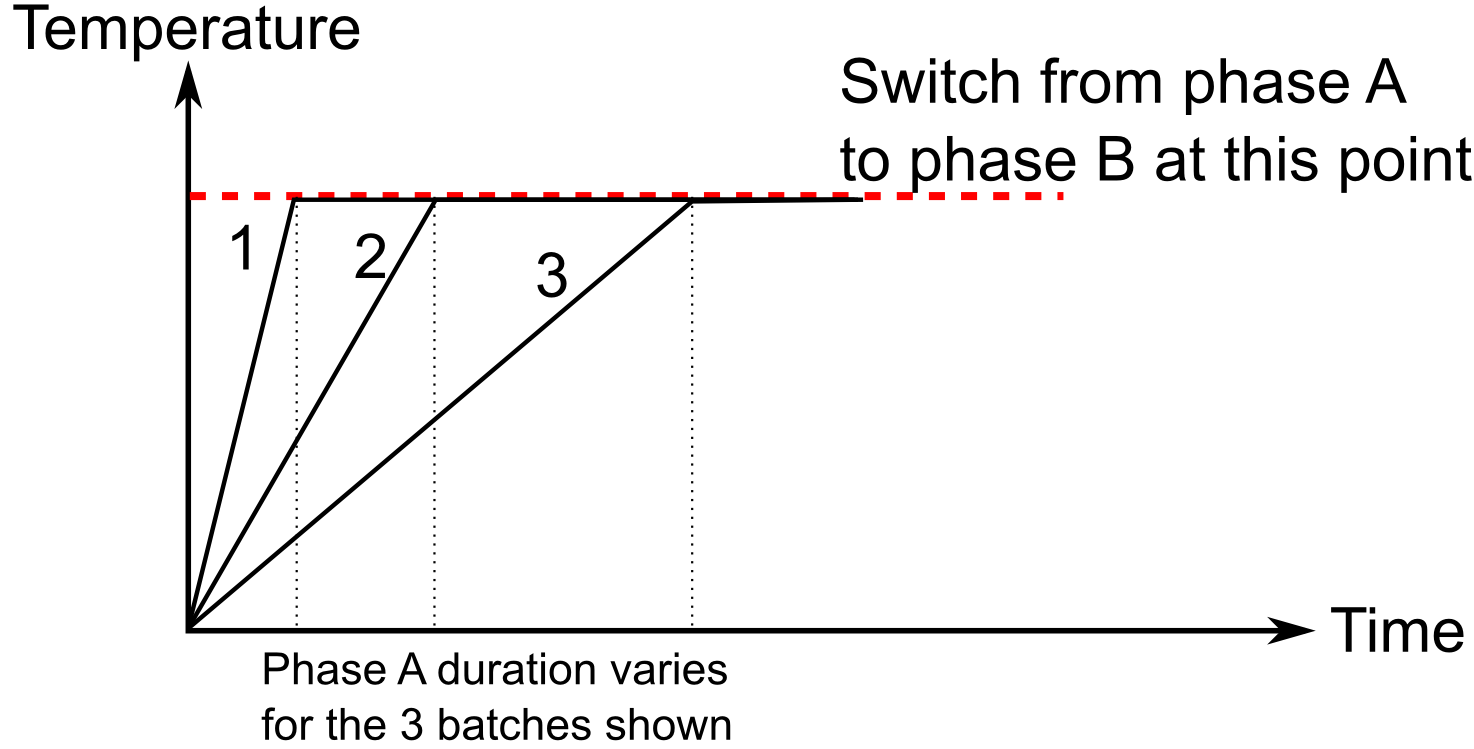
\includegraphics[width=0.7\textwidth]{images/alignment-due-to-phase-switching.png}
					\end{center}
		\end{itemize}
		\vspace{12pt}
		
	\column{0.3\textwidth}
	
		\begin{center}
			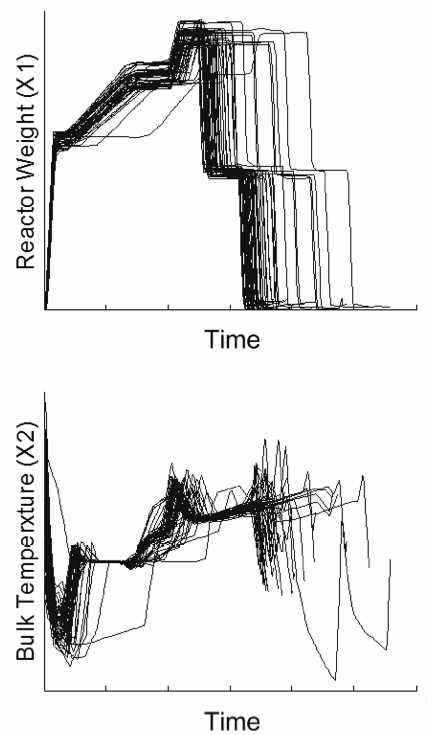
\includegraphics[width=\textwidth]{images/unaligned-trajectories-many-batches.png}
		\end{center}

		\small
		\textbf{Result}: similar trajectories of different duration
\end{columns}
\end{frame}

\begin{frame}\frametitle{Batch alignment: how to align}

Some automated tools are becoming available.  Best results still require case-specific knowledge.
\begin{itemize}
	
	\item	{\color{myGreen}{\emph{Data trimming}}}: throw out data points at start or end of each phase to match average duration.
	
			\begin{itemize}
				\item	\alert{Risk}:  most informative data often near start or end
			\end{itemize}
			
			\pause
	
	\item	{\color{myGreen}{\emph{Dynamic time warping}}}: stretch and shrink data to match a ``golden'' batch
	
			\begin{itemize}
				\item	Hard (impossible?) for real-time monitoring
			\end{itemize}
			
			\pause
	
	\item	{\color{myGreen}{\emph{Indicator variable}}}: find/create a monotonic variable within each phase and apply linear interpolation against it.
		
\end{itemize}

\end{frame}

\begin{frame}\frametitle{Batch alignment: aligning with an indicator}

\begin{itemize}
	
	\item	Good results if indicator is related to batch maturity
	
	\item	Adjust all other variables in phase against this indicator, and interpolate all batches to same number of \( J \) time points
	
	\item	Examples: 
			
			\begin{itemize}
				\item	temperature ramp
				
				\item	amount of raw material fed (semi-batch systems)
				
				\item	create a calculated variable, e.g. the total conversion
				
				\item	lance position in injection molding
			\end{itemize}
			
			\pause
	
	\item	Can be used for online, real-time monitoring (e.g. extrapolate temperature slope, use amount of material fed) \pause
	
	\item	Put the alignment information into \( Z \): very useful for diagnosis
\end{itemize}

\todo{Put some alignment diagrams from Cecilia's thesis here}

\end{frame}

%-------------------------------------------------
\section{Summary so far}
%-------------------------------------------------

\begin{frame}\frametitle{Value from batch process data}
\begin{enumerate}
	\item 	Learning more / confirming relationships
		
			\begin{itemize}
				\item 	understand between batch variation (overall scores, \( T^2 \), and SPE)
				\item 	understand within batch variation (instantaneous scores, \( T^2 \), and SPE)
			\end{itemize}
			
	\item 	Troubleshoot problems within a batch
	\item 	Optimize and improve: possible, but less likely in pharmaceutical applications
	\item 	Predictions: final quality attributes, endpoint
	\item 	Monitoring: can allow for early release to next stage
	
\end{enumerate}
\end{frame}
